\documentclass[12pt,letterpaper,oneside,titlepage]{article}
\usepackage[latin1]{inputenc}
\usepackage{amsmath}
\usepackage{amsfonts}
\usepackage{amssymb}
\usepackage{graphicx}
\usepackage[letterpaper, portrait, margin=.5in]{geometry}
\usepackage{lscape}
\usepackage{tikz}
\usetikzlibrary{matrix,calc}
\usepackage{color}
\usepackage{tabto}
\usepackage{pgfplots}



\usepackage[]{hyperref}
\hypersetup{
%	pdftitle={Tio Cash's Sort of Primes},
%	pdfauthor={Scott \textbf{``Cash''} Fields},
%	pdfsubject={Tio Cash's Sort of Primes},
	%pdfkeywords={keyword1, keyword2},
	bookmarksnumbered=true,     
	bookmarksopen=true,         
	bookmarksopenlevel=1,       
	colorlinks=true,   
	allcolors=blue,        
	pdfstartview=Fit,           
	pdfpagemode=UseOutlines,    % this is the option you were lookin for
%	pdfpagelayout=TwoPageRight
}
%%%%%%%%%%%%%%%%%%%%%%%%%%%%
%%%%%%%%%%%%%%%%%%%%%%%%%%%%
%%%%%%%%% cube pile %%%%%%%%%%%%%
%\documentclass[parskip]{scrartcl}
%\usepackage[margin=15mm,landscape]{geometry}
%\usepackage{tikz}
\usepackage{keyval}
\usepackage{ifthen}
%====================================
%emphasize vertices --> switch and emph style (e.g. thick,black)
%====================================
\makeatletter
% Standard Values for Parameters
\newcommand{\tikzcuboid@shiftx}{0}
\newcommand{\tikzcuboid@shifty}{0}
\newcommand{\tikzcuboid@dimx}{3}
\newcommand{\tikzcuboid@dimy}{3}
\newcommand{\tikzcuboid@dimz}{3}
\newcommand{\tikzcuboid@scale}{1}
\newcommand{\tikzcuboid@densityx}{1}
\newcommand{\tikzcuboid@densityy}{1}
\newcommand{\tikzcuboid@densityz}{1}
\newcommand{\tikzcuboid@rotation}{0}
\newcommand{\tikzcuboid@anglex}{0}
\newcommand{\tikzcuboid@angley}{90}
\newcommand{\tikzcuboid@anglez}{225}
\newcommand{\tikzcuboid@scalex}{1}
\newcommand{\tikzcuboid@scaley}{1}
\newcommand{\tikzcuboid@scalez}{sqrt(0.5)}
\newcommand{\tikzcuboid@linefront}{black}
\newcommand{\tikzcuboid@linetop}{black}
\newcommand{\tikzcuboid@lineright}{black}
\newcommand{\tikzcuboid@fillfront}{white}
\newcommand{\tikzcuboid@filltop}{white}
\newcommand{\tikzcuboid@fillright}{white}
\newcommand{\tikzcuboid@shaded}{N}
\newcommand{\tikzcuboid@shadecolor}{black}
\newcommand{\tikzcuboid@shadeperc}{25}
\newcommand{\tikzcuboid@emphedge}{N}
\newcommand{\tikzcuboid@emphstyle}{thick}

% Definition of Keys
\define@key{tikzcuboid}{shiftx}[\tikzcuboid@shiftx]{\renewcommand{\tikzcuboid@shiftx}{#1}}
\define@key{tikzcuboid}{shifty}[\tikzcuboid@shifty]{\renewcommand{\tikzcuboid@shifty}{#1}}
\define@key{tikzcuboid}{dimx}[\tikzcuboid@dimx]{\renewcommand{\tikzcuboid@dimx}{#1}}
\define@key{tikzcuboid}{dimy}[\tikzcuboid@dimy]{\renewcommand{\tikzcuboid@dimy}{#1}}
\define@key{tikzcuboid}{dimz}[\tikzcuboid@dimz]{\renewcommand{\tikzcuboid@dimz}{#1}}
\define@key{tikzcuboid}{scale}[\tikzcuboid@scale]{\renewcommand{\tikzcuboid@scale}{#1}}
\define@key{tikzcuboid}{densityx}[\tikzcuboid@densityx]{\renewcommand{\tikzcuboid@densityx}{#1}}
\define@key{tikzcuboid}{densityy}[\tikzcuboid@densityy]{\renewcommand{\tikzcuboid@densityy}{#1}}
\define@key{tikzcuboid}{densityz}[\tikzcuboid@densityz]{\renewcommand{\tikzcuboid@densityz}{#1}}
\define@key{tikzcuboid}{rotation}[\tikzcuboid@rotation]{\renewcommand{\tikzcuboid@rotation}{#1}}
\define@key{tikzcuboid}{anglex}[\tikzcuboid@anglex]{\renewcommand{\tikzcuboid@anglex}{#1}}
\define@key{tikzcuboid}{angley}[\tikzcuboid@angley]{\renewcommand{\tikzcuboid@angley}{#1}}
\define@key{tikzcuboid}{anglez}[\tikzcuboid@anglez]{\renewcommand{\tikzcuboid@anglez}{#1}}
\define@key{tikzcuboid}{scalex}[\tikzcuboid@scalex]{\renewcommand{\tikzcuboid@scalex}{#1}}
\define@key{tikzcuboid}{scaley}[\tikzcuboid@scaley]{\renewcommand{\tikzcuboid@scaley}{#1}}
\define@key{tikzcuboid}{scalez}[\tikzcuboid@scalez]{\renewcommand{\tikzcuboid@scalez}{#1}}
\define@key{tikzcuboid}{linefront}[\tikzcuboid@linefront]{\renewcommand{\tikzcuboid@linefront}{#1}}
\define@key{tikzcuboid}{linetop}[\tikzcuboid@linetop]{\renewcommand{\tikzcuboid@linetop}{#1}}
\define@key{tikzcuboid}{lineright}[\tikzcuboid@lineright]{\renewcommand{\tikzcuboid@lineright}{#1}}
\define@key{tikzcuboid}{fillfront}[\tikzcuboid@fillfront]{\renewcommand{\tikzcuboid@fillfront}{#1}}
\define@key{tikzcuboid}{filltop}[\tikzcuboid@filltop]{\renewcommand{\tikzcuboid@filltop}{#1}}
\define@key{tikzcuboid}{fillright}[\tikzcuboid@fillright]{\renewcommand{\tikzcuboid@fillright}{#1}}
\define@key{tikzcuboid}{shaded}[\tikzcuboid@shaded]{\renewcommand{\tikzcuboid@shaded}{#1}}
\define@key{tikzcuboid}{shadecolor}[\tikzcuboid@shadecolor]{\renewcommand{\tikzcuboid@shadecolor}{#1}}
\define@key{tikzcuboid}{shadeperc}[\tikzcuboid@shadeperc]{\renewcommand{\tikzcuboid@shadeperc}{#1}}
\define@key{tikzcuboid}{emphedge}[\tikzcuboid@emphedge]{\renewcommand{\tikzcuboid@emphedge}{#1}}
\define@key{tikzcuboid}{emphstyle}[\tikzcuboid@emphstyle]{\renewcommand{\tikzcuboid@emphstyle}{#1}}
% Commands
\newcommand{\tikzcuboid}[1]{
	\setkeys{tikzcuboid}{#1} % Process Keys passed to command
	\pgfmathsetmacro{\vectorxx}{\tikzcuboid@scalex*cos(\tikzcuboid@anglex)}
	\pgfmathsetmacro{\vectorxy}{\tikzcuboid@scalex*sin(\tikzcuboid@anglex)}
	\pgfmathsetmacro{\vectoryx}{\tikzcuboid@scaley*cos(\tikzcuboid@angley)}
	\pgfmathsetmacro{\vectoryy}{\tikzcuboid@scaley*sin(\tikzcuboid@angley)}
	\pgfmathsetmacro{\vectorzx}{\tikzcuboid@scalez*cos(\tikzcuboid@anglez)}
	\pgfmathsetmacro{\vectorzy}{\tikzcuboid@scalez*sin(\tikzcuboid@anglez)}
	\begin{scope}[xshift=\tikzcuboid@shiftx, yshift=\tikzcuboid@shifty, scale=\tikzcuboid@scale, rotate=\tikzcuboid@rotation, x={(\vectorxx,\vectorxy)}, y={(\vectoryx,\vectoryy)}, z={(\vectorzx,\vectorzy)}]
		\pgfmathsetmacro{\steppingx}{1/\tikzcuboid@densityx}
		\pgfmathsetmacro{\steppingy}{1/\tikzcuboid@densityy}
		\pgfmathsetmacro{\steppingz}{1/\tikzcuboid@densityz}
		\newcommand{\dimx}{\tikzcuboid@dimx}
		\newcommand{\dimy}{\tikzcuboid@dimy}
		\newcommand{\dimz}{\tikzcuboid@dimz}
		\pgfmathsetmacro{\secondx}{2*\steppingx}
		\pgfmathsetmacro{\secondy}{2*\steppingy}
		\pgfmathsetmacro{\secondz}{2*\steppingz}
		\foreach \x in {\steppingx,\secondx,...,\dimx}
		{   \foreach \y in {\steppingy,\secondy,...,\dimy}
			{   \pgfmathsetmacro{\lowx}{(\x-\steppingx)}
				\pgfmathsetmacro{\lowy}{(\y-\steppingy)}
				\filldraw[fill=\tikzcuboid@fillfront,draw=\tikzcuboid@linefront] (\lowx,\lowy,\dimz) -- (\lowx,\y,\dimz) -- (\x,\y,\dimz) -- (\x,\lowy,\dimz) -- cycle;
				
			}
		}
		\foreach \x in {\steppingx,\secondx,...,\dimx}
		{   \foreach \z in {\steppingz,\secondz,...,\dimz}
			{   \pgfmathsetmacro{\lowx}{(\x-\steppingx)}
				\pgfmathsetmacro{\lowz}{(\z-\steppingz)}
				\filldraw[fill=\tikzcuboid@filltop,draw=\tikzcuboid@linetop] (\lowx,\dimy,\lowz) -- (\lowx,\dimy,\z) -- (\x,\dimy,\z) -- (\x,\dimy,\lowz) -- cycle;
			}
		}
		\foreach \y in {\steppingy,\secondy,...,\dimy}
		{   \foreach \z in {\steppingz,\secondz,...,\dimz}
			{   \pgfmathsetmacro{\lowy}{(\y-\steppingy)}
				\pgfmathsetmacro{\lowz}{(\z-\steppingz)}
				\filldraw[fill=\tikzcuboid@fillright,draw=\tikzcuboid@lineright] (\dimx,\lowy,\lowz) -- (\dimx,\lowy,\z) -- (\dimx,\y,\z) -- (\dimx,\y,\lowz) -- cycle;
			}
		}
		\ifthenelse{\equal{\tikzcuboid@emphedge}{Y}}%
		{\draw[\tikzcuboid@emphstyle](0,\dimy,0) -- (\dimx,\dimy,0) -- (\dimx,\dimy,\dimz) -- (0,\dimy,\dimz) -- cycle;%
			\draw[\tikzcuboid@emphstyle] (0,0,\dimz) -- (0,\dimy,\dimz) -- (\dimx,\dimy,\dimz) -- (\dimx,0,\dimz) -- cycle;%
			\draw[\tikzcuboid@emphstyle](\dimx,0,0) -- (\dimx,\dimy,0) -- (\dimx,\dimy,\dimz) -- (\dimx,0,\dimz) -- cycle;%
		}%
		{}
	\end{scope}
}
\makeatother

%%%%%%%%%%%%%%%%%%%%%%%%%%%%
%%%%%%%%%%%%%%%%%%%%%%%%%%%%
% https://tex.stackexchange.com/questions/103123/links-do-not-lead-to-right-pages

\begin{document}
\author{Scott \textbf{``Cash''} Fields}
\title{Tio Cash's Sort of Primes}
\maketitle


%%%%%%%%%%%%%%%%%%%%%%%%%%%%%%%%%%%%%%%%%%%%%
%links in toc will not jump to abstract
%https://tex.stackexchange.com/questions/103123/links-do-not-lead-to-right-pages
%http://latex.org/forum/viewtopic.php?t=1205
%dedication
%http://gradschool.unc.edu/academics/thesis-diss/guide/ordercomponents.html


%%%%%%%%%%%%%%%%%%%%%%%%%%%%%%%%%%%%%%%%%%%%%

\begin{abstract}

	\textbf{ I have fought the good fight, I have finished the race, I have kept the faith.}

\end{abstract}	
\pagebreak

%%%%%%%%%%%%%%%%%%%
%%%%%%%%%%%%%%%%%%%%%%%%%%%%%%%%%%%%%%%%%%%%%%





%%%%%%%%%%%%%%%%%%%%%%%%%%%%%%%%
\section*{Acknowledgment}
%%\addcontentsline{toc}{section}{Acknowledgement}

Special thanks to Professor Hal Slice for two things:
\newline
\par
1) Teaching me the ability to count to infinity:
\hfill
\newline
\hspace*{12mm} 1 , 2 , 3 , . . . , K , K + 1
\newline
\par
2) Spending a summer outside of a classroom for numerous days and teaching
me how to
\newline
\hspace*{12mm} look for a formula vs. brute force inspection.


\pagebreak


\tableofcontents
%\addcontentsline{toc}{section}{Abstract}
%\addcontentsline{toc}{section}{Acknowledgment}

%%%%% Learn       %%%%%%%%%%%%%%%%%%%%%%%%%%%
%%%%%%%%%%%%%%%%%%%%%%%%%%%%%%%%


%%%%%%%%%%%%%%%%%%%%%%%%%%%%%%%%
%%%%%%%%%%%%%%%%%%%%%%%%%%%%%%%%
%%%%%%%%%%%%%%%%%%%%%%%%%%%%%%%%
%\section{Useful URL's}
%	\paragraph{FIRST TITLE}
	
%		\hfill
%\vspace{5mm} %5mm vertical space	

%	Hi
%	\paragraph{Para 1}
%	\hfill
%\vspace{5mm} %5mm vertical space
%	https://earthsci.stanford.edu/computing/unix/formatting/latexexample.php
%\vspace{5mm} %5mm vertical space
%	http://mally.stanford.edu/~sr/computing/latex-example.html
%\vspace{5mm} %5mm vertical space
%	http://www.electronics.oulu.fi/latex/examples/example\_1/
%\vspace{5mm} %5mm vertical space
%	https://en.wikibooks.org/wiki/LaTeX/Sample\_LaTeX\_documents
%	\vspace{5mm} %5mm vertical space
%https://www.sharelatex.com/learn/Main\_Page
%	\paragraph{Para 2 Ref Manuals}
%\hfill
%\vspace{5mm} %5mm vertical space
%http://tug.org/texinfohtml/latex2e.html
%\vspace{5mm} %5mm vertical space
%https://www.tug.org/utilities/plain/cseq.html
%\vspace{5mm} %5mm vertical space
%https://stuff.mit.edu/afs/athena/contrib/tex-contrib/beamer/pgf-1.01/doc/generic/pgf/version-for-tex4ht/en/pgfmanual.html#pgfmanualse9.html
%matrix
%https://tex.stackexchange.com/questions/300109/simple-visualization-of-3d-matrix
%cube
%https://tex.stackexchange.com/questions/29877/need-help-creating-a-3d-cube-from-a-2d-set-of-nodes-in-tikz/29882#29882
% quick ref
%https://www.library.caltech.edu/sites/default/files/latex-quickguide.pdf
%%%%%%%%%%%%%%%%%%%%%%%%%%%%%%
%\pagebreak
%\section{PNG}
%	\paragraph{Para 3 PNG} 
%	\vspace{5mm} %5mm vertical space
%	Graphics
%	
%%"firstXLS".png}
%%\includegraphics{"firstXLS".png}


%%%%%%%%%%%%%%%%%%%%%%%%%%%%%%%%
 %%\pagebreak
%%\begin{landscape}
%%\end{landscape}

%%%%%%%%%%%%%%%%%%%%%%%%%%%%%%%%
%%%%%%%%%%%%%%%%%%%%%%%%%%%%%%%%
%%%%%%%%%%%%%%%%%%%%%%%%%%%%%%%%
%%%%%%%%%%%%%%%%%%%%%%%%%%%%%%%%
%%%%%%%%%%%%%%%%%%%%%%%%%%%%%%%%
%%%%%%%%%%%%%%%%%%%%%%%%%%%%%%%%
%%%%%%%%%%%%%%%%%%%%%%%%%%%%%%%%
\pagebreak
\section{Why ?}
\subsection{Why ?  - And A Reason}
\par
\tab A long , long time ago in a far away land called the auto industry , I learned how 
collate and sort data. In a mythical story , there was once a problem with a
hood's rubber bumper. It was too thin. So , the hood fit was too low. Well , 
in order to ensure customer quality , we (QC) had to go out and canvass the
property to separate the good vehicles from the suspect vehicles. A sorting
process.
\\ 
\par
So , teams of guys would lift the hoods on all the vehicles and
replace the suspect part with a good part. Now , the list of vehicles was
like swiss cheese. There were old vehicles , new vehicles , good vehicles ,
and suspect vehicles. We had to record the last six digits
(the serial number) of the VIN (Vehicle Identification Number).
\\ 
\par
 There were numerous pieces paper with hand written data with unordered
serial numbers.
\\ 
\par
I watched one guy manually take all the serial numbers and check off each
serial number against a preprinted sheet with boxes number from 000
(zero , zero , zero) to 099 (zero , nine , nine). This was a range of one
hundred vehicles. The page heading would be the first three digits of the
hundred-thousands (ex: 110xxx). Finally , after all the scraps of paper were
accounted for. There was still swiss cheese. Some VINs were unaccounted for , they 
had already been shipped to the customer. So , a new list of the
missing VIN's was created to find and correct those vehicles.
\\
\par
 In real life this is done every day , what to sort out , and what to sort in.
\\
\par
 It's all just \textbf{data}. And you make the necessary rules to sort it . . .
\\
\subsection{The Goal}
\vspace*{2mm}
\par 
\tab 
The goal is: To have more fun . . . 
\\
\par 
This is a lighthearted look at numbers and specifically prime numbers.



\pagebreak
\section{The Data}

\par
\tab
Looking for prime numbers , there are all kinds of formulas with complex solutions. You can Google ``prime numbers" and find all kinds of information about \textbf{complex} upper level math formulas.
\\
\par A rough definition for primes is: 
A positive integer that is not divisible without remainder by any integer except itself and 1.
\\
\par I wanted to find a simple solution. A working\textendash man's theory. A simple blue collar working man's \mbox{solution}.
\\
\par
The goal is to find a \textbf{sort} or formula(s) that can easily identify these numbers.
\\
\par 
What drove me in this direction was after looking at prime numbers for a long time , I ask the question ``What make a number \textbf{not prime} , and how can I find them?'' I turned the coin over and looked at the reverse side. Then I flipped it back over to the obverse .
\\
\par 
The common thread is these numbers all end in 1 , 3 , 7 , 9.
\\
\par 
This is where we will create ``wild\textendash card'' numbers.  So, any numbers that end
in 3 (13, 23, 33, 43, . . . , 113, 123, . . . , 111003) can all be grouped together.  In
real life we group and sub\textendash group collections of things all sorts of things.
All the blue marbles.  All the diesel engines.  All the red trucks with
manual transmissions.  All the big birds.  All the white buffalo. 
\\
\par
 Sorting in and sorting out things.  Numbers are the same thing, there is nothing
special about a group of numbers.  All numbers that end with 3, could be
categorized as \textbf{*3} (wild\textendash card three).  This creates a sorting of the numbers
with a least significant digit of 3.
\\
We can represent the number 113 as *3 or 1127 as *7.     
\\

All numbers no matter how big , that end with one of the above digits ; 1 , 3 , 7 , 9 are a candidate
to be a prime number. 


\pagebreak
\section{The Data In Arts And Charts}

\par
\tab While examining primes , I used a simple EXCEL spreadsheet to create a graph.
I eliminated 2 (two) and 5 (five) ; and I will get to that later. I just wanted to look at digits ; *1 , *3 , *7 , *9.
I entered those prime numbers into a table and created a simple EXCEL graph. 
\\What I saw intrigued me.

%%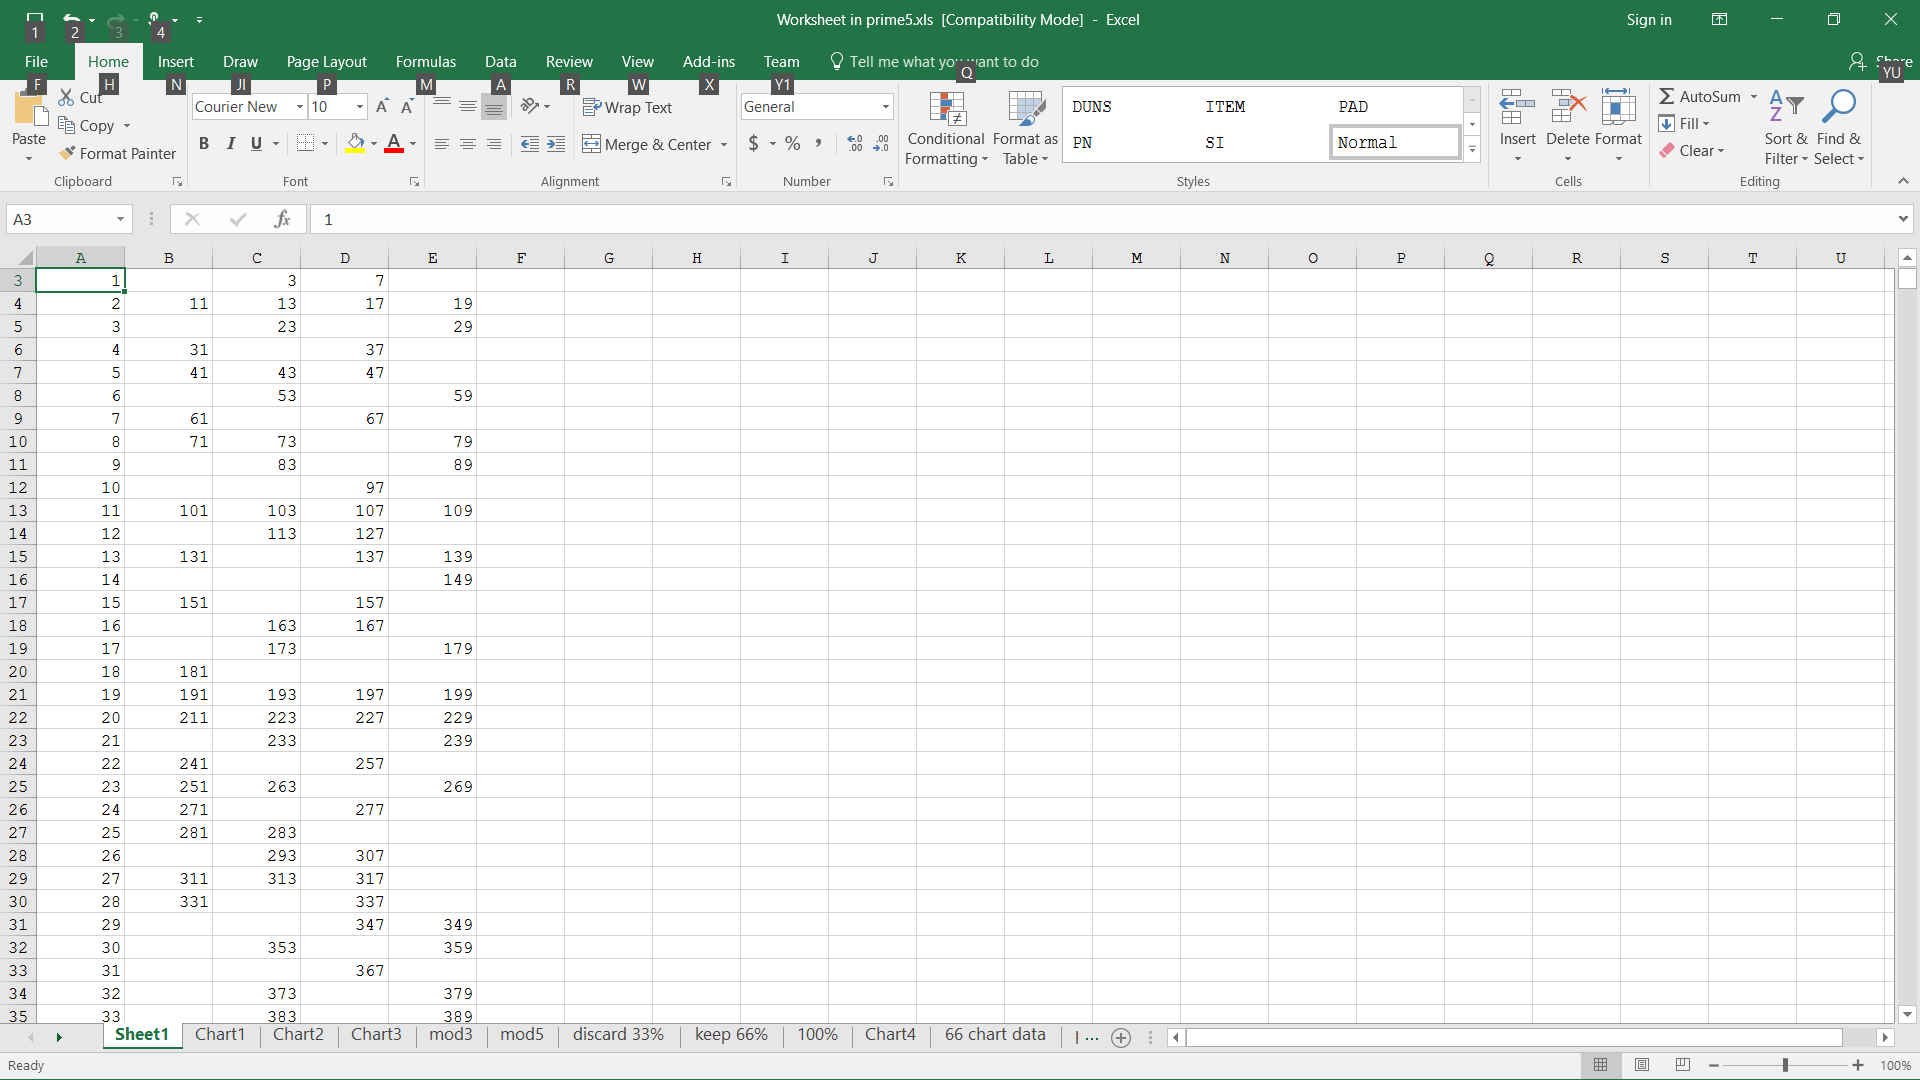
\includegraphics{00b broken line chart data.png}     
\begin{figure}[h]
	\centering
	\includegraphics[width=180mm, height=150mm]{"00b broken line chart data".png}
	\caption{Data for *1 *3 *7 *9 Prime Numbers}
\end{figure}
\pagebreak



\par 
 So , here is the graph. It is a broken line graph. I kind of expected that.
But what intrigued me was the little squiggles in the lines. It looked like a spiral.

%%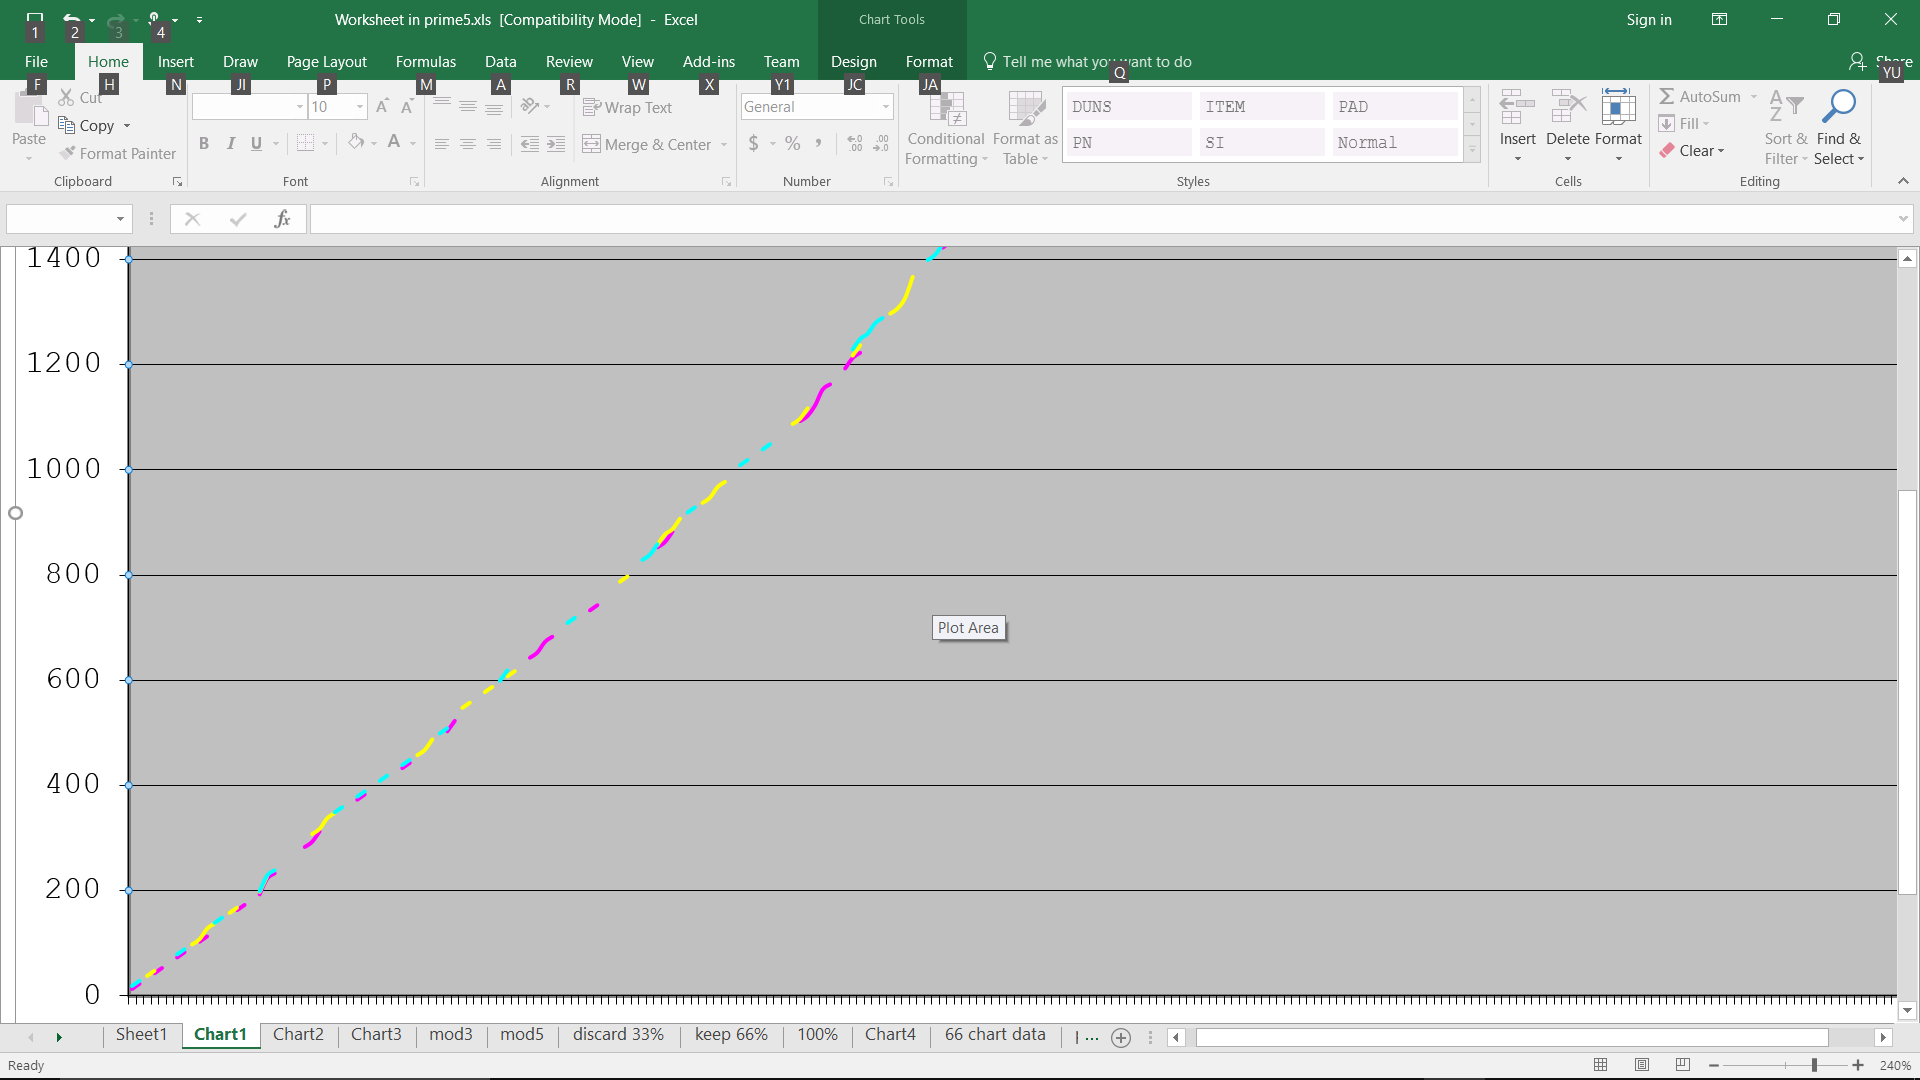
\includegraphics{00a broken line chart.png}  
\begin{figure}[h]
	\centering
	\includegraphics[width=180mm, height=150mm]{"00a broken line chart".png}
	\caption{Squiggle Graph for *1 *3 *7 *9 Prime Numbers}
\end{figure}
\pagebreak   



\section{Scrutinize The Numbers By Inspection}

\par 
\tab The next several charts will show some EXCEL sheets that distill down the view of all numbers to get closer to wild\textendash card numbers.
\\
\par This chart shows all numbers by the mod function (=MOD (number, divisor)), which will return the remainder of integer division. These cells are conditionally formated to be yellow if the value is zero (0). This shows were a number can be divided by some other number without a remainder. 
\\
\par Column C is the focus of the division , the painted cells are grouped by color for numbers *1 , *3 , *7 , *9. Wild\textendash card numbers.
\\
\par Columns D , E , F , . . . are the remainder values. 
\\
\par The gray painted cells relate to the the square root function. Column B is the value of the nearest perfect square. There is a pattern  between the integer number of the perfect square and the remainders  of its neighbors above and below.
%%01 mod all.pn
\begin{figure}[h]
	\centering
	\includegraphics[width=180mm, height=150mm]{"01 mod all".png}
	\caption{Mod All Numbers}
\end{figure}
\pagebreak  


\par 
Lets sort out the even numbers any *2 , *4  , *6 , *8 , *0.
\\
\par 
This will give a closer look at the odd numbers. Same chart just odd numbers only.
\\
\par We are drilling down , we are starting to sort out the unwanted.
%%    02 mod odd.png	
\begin{figure}[h]
	\centering
	\includegraphics[width=180mm, height=150mm]{"02 mod odd".png}
	\caption{Mod Odd Numbers}
\end{figure}
\pagebreak  

\par 
Here is a close up of the prior graphic. 
\\
\par 
Look at 33 , it can be 3 x 11 or 11 x 3
\\
\par 
35 shows 5 x 7 and 7 x 5 , they are situated on both sides of 6. The square root of 36.
\\
\par 
One last look , 49 (circled) is 7 x 7. No matter what.
\\
\par 
We only need to look as far as the square root to determine if a number is prime.

\begin{figure}[h]
	\centering
	\includegraphics[width=180mm, height=150mm]{"04 mod odd sqrt B".png}
	\caption{Mod Odd Square Root B}
\end{figure}
\pagebreak  

%%%%%%%%%%%%%%%%%%%%%%%%
%%%%%%%%%%%%%%%%%%%%%%%%%
\par 
Right side of square root redundant.
\\
\par 
Before I get too far ahead of myself , the right side of the square root can be eliminated.
It is just the inverse of the left side. An example is (7 x 11) the same as (11 x 7). They are mirror images on both sides of the square root.
%%"04 mod odd sqrt".png
\begin{figure}[h]
	\centering
	\includegraphics[width=180mm, height=150mm]{"04 mod odd sqrt".png}
	\caption{Mod Odd Square Root}
\end{figure}
\pagebreak


%%%%%%%%%%%%%%%%%%%%%%
%%\subsection[Sort out 5]{title sort}
%% \\
\par 
Lets sort out the *5.
\\
\par 
I still have 2 and 5 , but I will get rid of them soon.
\\
\par 
This will give a larger view of the prior graphic. Here the color coding is getting close.
If you look closely the only yellow cells are in column E and the ending column of the mod function. Yes , I know this is all manual. 
\\
\par 
Here is the start of the primes with color coding by the least significant digit.
%%02 mod odd 2b.png     
\begin{figure}[h]
	\centering
	\includegraphics[width=180mm, height=150mm]{"02 mod odd 2b".png}
	\caption{Mod Odd Numbers B}
\end{figure}
\pagebreak  



\par There are eight separate formulas that can color code the numbers on the prior graphics.
%%"03 formula".png
\begin{figure}[h]
	\centering
	\includegraphics[width=180mm, height=150mm]{"03 formula".png}
	\caption{The Formula by Color}
\end{figure}
\pagebreak  

\section{2 And 5 Are Out}
\par 
\tab At this point lets look at 2 (two) and 5 (five).
\\
\par 
Both of these number are each a one shot , they only occur once 
as the least significant digit.
\\
It is extraneous data , sort them out.
\\
\subsection{2 - Deuces Are Wild}
\par 
\tab Two (2) is the only even number prime number. 
All subsequent even numbers are just a multiple of two (2). 
There will never be any number that is *2 greater than 2 that can be prime.
\\
\\
\begin{tabular}{|c|c|c|c|c|c|c|c|c|c|}
	\hline 
	1 & 2 & 3 & 4 & 5 & 6 & 7 & 8 & 9 & 10 \\ 
	\hline 
	2 & 4 & 6 & 8 &10  &12  &14  &16  &18 & 20 \\ 
	\hline 
\end{tabular}  
\\

\par 
The top row is the start of integer values. The bottom row is the result of multiplication by two (2)  ; all even digits.
All divisible by two (2).
%%%%%%%%%%%%
\subsection{5 - Five Is Alone}
\par 
\tab Five (5) is just like two (2) there is only one prime that will end with a five. All the rest are multiples of five (5). There will never be any number that is *5 greater than five (5) that can be prime.
\\
\\
\begin{tabular}{|c|c|c|c|c|c|c|c|c|c|}
	\hline 
	1 & 2 & 3 & 4 & 5 & 6 & 7 & 8 & 9 & 10 \\ 
	\hline 
	5 & 10 & 15 & 20 & 25  &30  &35  &40  &45 & 50 \\ 
	\hline 
\end{tabular}  
\\

\par 
The top row is the start of integer values. The bottom row is the result of multiplication by. Any even* number time five (5) will give a *0 number. Any *odd number times five (5) will give a *5 number. 
\\
\\
Remember wild\textendash card numbers.
\pagebreak




\section{How And Why Can We Discard Numbers}
\par 
\tab In the real world we make sorts of rules for all kinds of different situations. 
\\
\par 
The first that comes to mind is the old MS-DOS ``dir'' command.
\\
 We could sort files with ``dir a*.com'' - give me a list of all files that starts with ``a'' , and are any length or values and have a ``com'' extension.
\\
\par 
Next ,  in a TSO Mainframe File Edit , is a command like `` sort 12 15 a 23 34 d 16 18 a '' - sort columns 12 to 15 ascending , and then 23 to 34 descending , and finally 16 to 18 ascending.
\\
\par 
In another program we could say:
\\
`` define pick/a1 = if ((stkm = edit(******9) = `r') or (stkm = edit(*****9*) = `r')) then `Y' else ` ' ;  ''
\\ 
if pick equals ``Y'' (yes) then later select (sort in) these records. Do not select (sort out) the blank `` '' records.
\\
\par 
Finally , my favorite and hopefully best argument.
\\
\par 
In any good text editor is a thing called regex (regular expression). It allow for pattern matching in a file.
 I wont go to deep here ; but this is a perfect example of the \underline{text (read: data) tool being developed for the need.}
\\
\par 
In my text editor KEDIT an example would be: `` locate reg /z?c/ ''. Locate any string that starts with a ``z'' and has ``any character'' and ends with a ``c''.
\\
\par
Google `` regular expression '' for real fun! Read the history.
\\
\par 
All the above examples are really a sort ; sorting out what we don't want and soring in what we want to keep. Each is a different tool based on the data.
\\
\par



\pagebreak 
%%%%%%%%%%%%D
\section{Let Us Go Hunt For The Sort And Formula(s)}
\par 
\tab In the below slide are \underline{\textbf{all}} the possible integers sorted by there least significant digit. 
\\
\par
Once again remember wild\textendash card numbers.
\\
\par 
There are ten piles of numbers.  From *0 , *1 , *2 ,  . . . , *9.
\\
\par
Yellow colored are even numbers , and green colored are odd numbers.
\\
%%"50 wild-card".png
\begin{figure}[h]
	\centering
	\includegraphics[width=180mm, height=150mm]{"50 wildcard".png}
	\caption{Color Code Yellow = Even And Green = Odd }
\end{figure}

\pagebreak  


\par 
Next , let's sort the even (yellow) to the left ; and odd (green) to the right.
%%"52 wildcard".png
\begin{figure}[h]
	\centering
	\includegraphics[width=180mm, height=150mm]{"52 wildcard".png}
	\caption{Even Odd Sort By Color}
\end{figure}

\pagebreak

\par 
Next move the *5 next to the yellow and in front of the *1. This is an sort based on eliminating the *5 from above.
%%"54 wildcard".png
\begin{figure}[h]
\centering
\includegraphics[width=180mm, height=150mm]{"54 wildcard".png}
\caption{Move *5}
\end{figure}
\pagebreak

\par 
The color of *5 in now yellow , we have discarded it.
\par
This leaves the numbers *1 and *3 and *7 and *9 for the hunt.
%%"56 wildcard".png
\begin{figure}[h]
\centering
\includegraphics[width=180mm, height=150mm]{"56 wildcard".png}
\caption{Change *5 to Yellow}
\end{figure}
\pagebreak

\par 
What is unique about these numbers is the location to nearby 5 (five) and zero (0).
\\
\par 
It appears that all prime numbers hover around *5 and *0.
\\
\par 
So , 
\\
\par
\begin{tabular}{rrrr}
%	\hline 
	\rule[-1ex]{0pt}{2.5ex}  \hspace{1cm}&*1&is&*0 + 1\\ 
%	\hline 
	\rule[-1ex]{0pt}{2.5ex}  \hspace{1cm}&*3&is& *5 - 2\\ 
%	\hline 
	\rule[-1ex]{0pt}{2.5ex}  \hspace{1cm}&*7&is&*5 + 2\\ 
%	\hline 
	\rule[-1ex]{0pt}{2.5ex}  \hspace{1cm}&*9&is& *0 - 1\\ 
%	\hline 
\end{tabular} 
%%"58 wildcard 5+-2 or 0+-1".png
\begin{figure}[h]
\centering
\includegraphics[width=180mm, height=150mm]{"58 wildcard 5+-2 or 0+-1".png}
\caption{*5 +/- 2 or *0 +/- 1}
\end{figure}
\pagebreak

\par
We can further sort out one-third (1/3) of the remaining numbers. Every third occurrence will be a multiple of three (3).
I promise to get you to the end. Trust me  . . .
\\
%%"60 wildcard 5+-2 or 0+-1 3rd".png
\begin{figure}[h]
\centering
\includegraphics[width=180mm, height=150mm]{"60 wildcard 5+-2 or 0+-1 3rd".png}
\caption{Eliminate One-Third of *1 , *3 , *7 , *9}
\end{figure}
\pagebreak


\par 
So we are left with a patch of numbers to look at.
\\
\par
 Some serious number theorist will disagree but we have eliminated a percentage of numbers. 
\\
\par 50\% for the *even numbers , 10 \% for the *5 numbers. Then 33\% of each of the rest. 
\\
\par 
So 33\% of 10\% for four occurrences. .333 x .10 x 4 = .1332 or $\approx$ 13.32\%
\\
\par 
Added all up is $\approx$ 73.32\% are gone. We have to look at the balance , $\approx$ 26.68\% of the numbers.
\\	
\par 
Take 8 $\div$ 30 = $\approx$ 26.68\%
%%"62 wildcard 5+-2 or 0+-1 3rd".png
\begin{figure}[h]
\centering
\includegraphics[width=180mm, height=150mm]{"62 wildcard 5+-2 or 0+-1 3rd".png}
\caption{\% Of What Is Left}
\end{figure}
\pagebreak




%%"64 wildcard 5+-2 or 0+-1 3rd".png
\begin{figure}[h]
\centering
\includegraphics[width=180mm, height=150mm]{"64 wildcard 5+-2 or 0+-1 3rd".png}
\caption{Just Another View Of The World}
\end{figure}
\pagebreak


\par 
Let's zoom in on *3. 
\\
\par 
Just to be clear from here on out when you see and read (3)(10) think the first four primes (1)(2)(3)(5) . 
\par  
So , 1 x 2 x 3 x 5 (1 times 2 times 3 times 5). 
\\
\par 
The graphics shows the formulas stacked three high , and for the results for n = 0 , 1 , 2 , 3 and 4.
\\ 
\\
\begin{tabular}{r|r|r}
\colorbox{yellow}{ 3 + n(3)(10) } & \colorbox{green}{ 13 + n(3)(10) }  & \colorbox{green}{ 23 + n(3)(10) } \\ 
\end{tabular} 
\\
\par 
The yellow cells are divisible by three (3). These are the one-third that we can eliminate.
The green cells are the focus of our search. 
\\	
\par 
These formulas will give all *3 numbers for n = 0 , 1 , 2 , 3 , . . . , $\infty$ . 	
\\

%%"66 wildcard forumla 01 for 3".png
\begin{figure}[h]
\centering
\includegraphics[width=180mm, height=150mm]{"66 wildcard forumla 01 for 3".png}
\caption{Zoom In On *3}
\end{figure}
\pagebreak
	


%%%%%%%%%%%%%%%%%%%%%%%
\par 
Just for clarification.
%%"68 wildcard forumla 02 for 3".png
\begin{figure}[h]
	\centering
	\includegraphics[width=180mm, height=150mm]{"68 wildcard forumla 02 for 3".png}
	\caption{Zoom In On *3 Formulas Only}
\end{figure}
\pagebreak


\par 
Here is another view of the *3 formulas and the results.
%%"70 wildcard forumla 03 for 3".png
\begin{figure}[h]
	\centering
	\includegraphics[width=180mm, height=150mm]{"70 wildcard forumla 03 for 3".png}
	\caption{Zoom In On *3 Formula Results Only}
\end{figure}
\pagebreak




\par 
Here are the *1 , * 3 , *7 , *9 numbers with the one-third number color coded yellow to eliminate the division by 3 portion.
\\ 
\par 
This same argument can be carried from *3 to the other numbers.
%%"72 wildcard formula to remove 3rds graph 02".png
\begin{figure}[h]
	\centering
	\includegraphics[width=180mm, height=150mm]{"72 wildcard formula to remove 3rds graph 02".png}
	\caption{0 +/- 1 and 5 +/-2 With Color}
\end{figure}
\pagebreak



\par 
Here are all the numbers from one (1) to thirty (30) with color coding for division by three (3).
%%"72 wildcard formula to show matrix all numbers".png
\begin{figure}[h]
	\centering
	\includegraphics[width=180mm, height=150mm]{"72 wildcard formula to show matrix all numbers".png}
	\caption{All Numbers By Color}
\end{figure}
\pagebreak


\par 
The next graphic is a matrix of formulas and an input of a value for n. And , the results.
\\
\par 
The top line is *1 , *3 , *7 , *9  or  0 + 1 , 5 - 2 , 5 + 2 , 0 - 1. 
The next three lines in the box are the formulas , every three lines below have the corresponding formulas.
The yellow painted cell are the ones that can be divided by three (3). The `n' heading in row 4 is the input value to the formulas. 
\\
\par 
It is funny , but note the numbers are all ten (10) apart. If you eliminate the yellow divisible by three (3) then it would appear that prime numbers \textbf{could} be ten (10) apart , followed by a gap of twenty (20)  apart for each column.
\\
\par 
So what do we have? A set of formulas that will list the possible prime numbers.

%%"80 100% of 1 3 7 9".png
\begin{figure}[h]
	\centering
	\includegraphics[width=180mm, height=150mm]{"80 100percent of 1 3 7 9".png}
	\caption{Show All Formulas And Results}
\end{figure}
\pagebreak

	
	

\par 
So , here are the formulas that can be sorted off and discarded.  No matter what value of `n' ; these are all divisible by three (3). I am going to allow the number three (3) be discarded at this time. I am just going to let it slip away.
%%"82 33% discard of 1 3 7 9".png
\begin{figure}[h]
	\centering
	\includegraphics[width=180mm, height=150mm]{"82 33percent discard of 1 3 7 9".png}
	\caption{Discard The One-third}
\end{figure}
\pagebreak


\par 
What is left are the unpainted cells. These are the keepers. Two-thirds of the *1 , *3 , *7 , *9 numbers. 
\\	
%%"84 66% keep of 1 3 7 9".png
\begin{figure}[h]
	\centering
	\includegraphics[width=180mm, height=150mm]{"84 66percent keep of 1 3 7 9".png}
	\caption{Keep The Two-thirds}
\end{figure}
\pagebreak


\par 
Now , here is a matrix of formulas that will give all numbers for `n' from 0 , 1 , 2 , 3 , . . . , $\infty$ . 
\\
\par 
The yellow painted cells are now the guys we want to take a closer look at.				
%%"86 just 1 3 7 9 formulas".png
\begin{figure}[h]
	\centering
	\includegraphics[width=180mm, height=150mm]{"86 just 1 3 7 9 formulas 2".png}
	\caption{Matrix of Formulas}
\end{figure}
\pagebreak
			
	
\par 
Here is the formula matrix. The ``initial matrix''  is from 1 to 30 as a constant.
\\
\par 
The ``Actual formulas in E , F , G'' matrix is the definition of the formulas in the respective columns.
\\
\par 
The input value is in cell E3. Just below `n'.
\\
\par 
The ``formulas for above result matrix'' is the human readable formula (a constant (1 to 30) plus the quantity of a variable `n' times (1*2*3*5)).
The ``result matrix'' will yield all numbers from zero (0) to infinity ($\infty$) .
\\ 
\par 
In this example n = 5.
%%"88 all odd and even formulas".png
\begin{figure}[h]
	\centering
	\includegraphics[width=180mm, height=150mm]{"88 all odd and even formulas".png}
	\caption{Formula Matrix}
\end{figure}
\pagebreak


\par 
The formula will also work for negative numbers of `n'. Here n = \textendash 1.
\\
\par 
So , the formulas are valid for numbers:
\\
\par 
 \textendash\space  $\infty$ , . . . , -3 , -2 , -1 , 0 , 1 , 2 , 3 , . . .  , + $\infty$
%%"88 negitive".png
\begin{figure}[h]
	\centering
	\includegraphics[width=180mm, height=150mm]{"88 negative".png}
	\caption{Formula Matrix With \textendash 1}
\end{figure}
\pagebreak


			
\par 
This graphic shows values of `n'  equal to 0 , 1 , 2 , 3 , 4 , 5. The results are from 1 to 180.

%%"90 all odd and even results 0-5".png
\begin{figure}[h]
	\centering
	\includegraphics[width=180mm, height=150mm]{"90 all odd and even results 0-5".png}
	\caption{Results For n = 0 to 5}
\end{figure}
\pagebreak



\par 
Here are the formulas that have \textbf{not} been sorted out with their color coding.
%%"92 1 3 7 9 formula".png
\begin{figure}[h]
	\centering
	\includegraphics[width=180mm, height=150mm]{"92 1 3 7 9 formula".png}
	\caption{Sorted In Formulas by Color}
\end{figure}
\pagebreak

\pagebreak
\section{The Cash Pile}
\subsection{Matrix}
\par 
Here is the full matrix with the possible primes painted in yellow. We have eliminated any 
\\
 *even , * (divisible by 3) , and *5.
\\
\\
Our formula has ( 1 x 2 x 3 x 5) the first four (4) primes. So , later when we start looking for prime we can start at seven (7). 
\\
\\
The eight equations will only work for the remaining numbers that we want to search threw. 
\\
%%%%%   LEARN     %%%%%%%%%%%%%%%%%%%%%
%%%%%%%%%%%%%%%%%%%%%%%%%%%%%%%%

\begin{tikzpicture}[every node/.style={anchor=north east ,fill=white,minimum width=3cm,minimum height=15mm}]

\matrix (mA) [draw,matrix of math nodes]
{
	\colorbox{yellow}{ =1 + (n)(3)(10)}   &   \colorbox{yellow}{= 11 + (n)(3)(10) }   &     =21 + (n)(3)(10)   &    \\
	=2 + (n)(3)(10)   &   =12 + (n)(3)(10)    &     =22 + (n)(3)(10)   &    \\
	=3 + (n)(3)(10)   &   \colorbox{yellow}{ =13 + (n)(3)(10) }   &   	\colorbox{yellow}{ =23 + (n)(3)(10) }  &    \\
	=4 + (n)(3)(10)   &   =14 + (n)(3)(10)    &     =24 + (n)(3)(10)   &    \\
	=5 + (n)(3)(10)   &   =15 + (n)(3)(10)    &     =25 + (n)(3)(10)   &    \\
	=6 + (n)(3)(10)   &   =16 + (n)(3)(10)    &     =26 + (n)(3)(10)   &    \\
	\colorbox{yellow}{ =7 + (n)(3)(10) }   &   \colorbox{yellow}{ =17 + (n)(3)(10) }    &     =27 + (n)(3)(10)   &    \\
	=8 + (n)(3)(10)   &   =18 + (n)(3)(10)    &     =28 + (n)(3)(10)   &    \\
	=9 + (n)(3)(10)   &   \colorbox{yellow}{ =19 + (n)(3)(10) }    &     \colorbox{yellow}{ =29 + (n)(3)(10) }   &    \\
	=10 + (n)(3)(10)  &   =20 + (n)(3)(10)   &     =30 + (n)(3)(10)    &  
	\colorbox{green}{n = \textendash $\infty$ , . . . ,  + $\infty$} \\
};



\pagebreak
\end{tikzpicture}
\pagebreak




%%%%%%%%%%%%%%%%%%%%%%%%%%%%%%%%%%
\subsection{Results}
\par 
Here are the results matrix with the possible primes painted in yellow. 
\\
This is for values of `n' =  -1 , 0 , 1 , 2.  The lowest number is in the top left corner , and the highest is in the bottom right corner.	
\\
\begin{tikzpicture}[every node/.style={anchor=north east ,fill=white,minimum width=1cm,minimum height=5mm}]
\small
\matrix (mA) [draw,matrix of math nodes]
{
	\colorbox{yellow}{(61)}   & \colorbox{yellow}{(71)} & (81)  &  \\
	%        (61)   & (71) & (81)  &  \\
	(62)   & (72) & (82)  &  \\ 
	(63)   & \colorbox{yellow}{(73)} & \colorbox{yellow}{(83)}  &  \\        
	%		(63)   & (73) & (83)  &  \\        
	(64)   & (74) & (84)  &  \\        
	(65)   & (75) & (85)  &  \\        
	(66)   & (76) & (86)  &  \\
	\colorbox{yellow}{(67)}   & \colorbox{yellow}{(77)} & (87)  &  \\        
	%		(67)   & (77) & (87)  &  \\        
	(68)   & (78) & (88)  &  \\ 
	(69)   & \colorbox{yellow}{(79)} & \colorbox{yellow}{(89)}  &  \\       
	%		(69)   & (79) & (89)  &  \\        
	(70)   & (80) & (90)  &  \colorbox{green}{n = 2} \\ 
};


\matrix (mB) [draw,matrix of math nodes] at ($(mA.south west)+(1,3)$)
{
	\colorbox{yellow}{(31)}   & \colorbox{yellow}{(41)} & (51)  &  \\        
	%       (31)   & (41) & (51)    &  \\
	(32)   & (42) & (52)    &  \\
	(33)   & \colorbox{yellow}{(43)} & \colorbox{yellow}{(53)}  &  \\    
	%		(33)   & (43) & (53)    &  \\
	(34)   & (44) & (54)    &  \\
	(35)   & (45) & (55)    &  \\
	(36)   & (46) & (56)    &  \\
	\colorbox{yellow}{(37)}   & \colorbox{yellow}{(47)} & (57)  &  \\
	%		(37)   & (47) & (57)    &  \\
	(38)   & (48) & (58)    &  \\
	(39)   & \colorbox{yellow}{(49)} & \colorbox{yellow}{(59)}  &  \\
	%		(39)   & (49) & (59)    &  \\
	(40)   & (50) & (60)    & \colorbox{green}{n = 1} \\  
};  

\matrix (mC) [draw,matrix of math nodes] at ($(mB.south west)+(1,3)$)
{
	\colorbox{yellow}{(1)}   & \colorbox{yellow}{(11)} & (21)  &  \\        
	(2)   & (12) & (22)  &  \\        
	(3)   & \colorbox{yellow}{(13)} & \colorbox{yellow}{(23)}  &  \\        
	(4)   & (14) & (24)  &  \\        
	(5)   & (15) & (25)  &  \\        
	(6)   & (16) & (26)  &  \\        
	\colorbox{yellow}{(7)}   & \colorbox{yellow}{(17)} & (27)  &  \\        
	(8)   & (18) & (28)  &  \\        
	(9)   & \colorbox{yellow}{(19)} & \colorbox{yellow}{(29)}  &  \\        
	(10) & (20) & (30) &  \colorbox{green}{n = 0} \\  
};


\matrix (mD) [draw,matrix of math nodes] at ($(mC.south west)+(1,3)$)	
{
	\colorbox{yellow}{(-29)}   & \colorbox{yellow}{(-19)} & (-9)  &  \\      
	%	(-29)   & (-19) & (-9) &  \\
	(-28)   & (-18) & (-8) &  \\
	(-27)   & \colorbox{yellow}{(-17)} & \colorbox{yellow}{(-7)}  &  \\    
	%	(-27)   & (-17) & (-7) &  \\
	(-26)   & (-16) & (-6) &  \\
	(-25)   & (-15) & (-5) &  \\
	(-24)   & (-14) & (-4) &  \\
	\colorbox{yellow}{(-23)}   & \colorbox{yellow}{(-13)} & (-3)  &  \\        
	%	(-23)   & (-13) & (-3) &  \\
	(-22)   & (-12) & (-2) &  \\
	(-21)   & \colorbox{yellow}{(-11)} & \colorbox{yellow}{(-1)}  &  \\        
	%	(-21)   & (-11) & (-1) &  \\
	(-20)   & (-10) & (0)  &  \colorbox{green}{n = - 1} \\
};                                   



\draw[dashed](mA.north east)--(mD.north east);
\draw[dashed](mA.north west)--(mD.north west);
\draw[dashed](mA.south east)--(mD.south east);
\normalfont 
\end{tikzpicture}
\pagebreak



\subsection{3D View Of The Cash Pile}
\par 
This is a view of the Cash Pile , it is a \textbf{small portion} of the numbers. The bottom face is a 3x10 matrix of the formulas. The right hand face is  `n' with each row the same value. In the interior are the results. This is just a \textbf{pile} of numbers that goes on forever  ; down (\textendash $\infty$ ) or up (+ $\infty$).
\\
\\
\begin{tikzpicture}
{
	\tikzcuboid{%
		shiftx=4cm,%
		shifty=0cm,%
		scale=0.90,%
		rotation=-83,%
		densityx=1,%
		densityy=1,%
		densityz=1,%
		dimx=10,%
		dimy=6,%
		dimy=10,%
		linefront=red!75!black,%
		linetop=red!50!black,%
		lineright=red!25!black,%
		fillfront=red!25!white,%
		filltop=red!50!white,%
		fillright=red!75!white%
	}
}
\end{tikzpicture}

\pagebreak
\subsection{Why Is The Pile Important ?}
\par 
\hspace*{6mm} The reverse of finding `n' is important to tell which formula has been matched. An integer value without a decimal remainder shows the intersection of the formula and a level of the pile. A *3 number can only match one formula.
\\
\par 
There can be a match from both formulas for different numbers on one level , or a missing level match. We will use this later to sort out some *3 data.

%%"92 1 3 7 9 formula".png
\begin{figure}[h]
	\centering
	\includegraphics[width=180mm, height=150mm]{"96 cash pile numbers".png}
	\caption{Sorted In Formulas by Color}
\end{figure}
\pagebreak







%%%%%%%%%%% %%%%%%%%%%%%%%%%%%%%%
%%%%%%%%%%%%%%%%%%%%%%%%%%%%%%%%
%%%%%%% y = mx + b %%%%%%%%%%%%%%%%%%%
%%%%%%%%%%%%%%%%%%%%%%%%%%%%%%%%%%
%%%% start here - show data - add pages - and move up
\section{y = mx + b} 
\par 
This graph is each of the eight formulas in the form of \textbf{y = mx + b}. 
\\Each pair of colors is part of a wild\textendash card number.
\\
% \colorbox{blue}{\textcolor{yellow}*1} is \colorbox{blue}{blue}
\large
\textbf{\textcolor{blue}{*1 is blue}} \space ; \space \textbf{\textcolor{red}{*3 is red}} 
\\
\textbf{\textcolor{black}{*7 is black}} \space ; \space \textbf{\textcolor{cyan}{*9 is cyan}} 
\\
\normalfont
\\
\begin{tikzpicture}[scale=\textwidth/8cm,]
\begin{axis}[
axis lines = middle,
title={Wild\textendash card Lines},
%xlabel={X},
%ylabel={Y},
xmin=-1, xmax=3,
ymin=-30, ymax=120,
xtick={-1,0,1,2,3},
ytick={0,10,20,30,40,50,60,70,80,90,100,110},
legend pos=north west,
ymajorgrids=true,
xmajorgrids=true,
grid style=dashed,
]
%%%%%%  1  %%%%%%%%%%%%
\addplot[
color=blue,
mark=.,
]
coordinates {
	(-1,-29)(0,1)(1,31)(2,61)(3,91)
};
%\legend{CuSO$_4\cdot$5H$_2$O}
%%%%%%  11 %%%%%%%%%%%%%
\addplot[
color=blue,
mark=.,
]
coordinates {
	(-1,-19)(0,11)(1,41)(2,71)(3,101)
};
%%%%%%%  13 %%%%%%%%%%%%
\addplot[
color=red,
mark=.,
]
coordinates {
	(-1,-17)(0,13)(1,43)(2,73)(3,103)
};
%%%%%%%  23  %%%%%%%%%%%%%
\addplot[
color=red,
mark=.,
]
coordinates {
	(-1,-7)(0,23)(1,53)(2,83)(3,113)
};
%%%%%  07  %%%%%%%%%%%%%%
\addplot[
color=black,
mark=.,
]
coordinates {
	(-1,-23)(0,7)(1,37)(2,67)(3,97)
};
%%%%%%  17 %%%%%%%%%%%%%
\addplot[
color=black,
mark=.,
]
coordinates {
		(-1,-13)(0,17)(1,47)(2,77)(3,107)
};

%%%%%%%%    19  %%%%%%%%%%%%%%%
\addplot[
color=cyan,
mark=.,
]
coordinates {
	(-1,-11)(0,19)(1,49)(2,79)(3,109)
};

%%%%%%%%%%%%%%%%%%%%%%%
%%%%%%%%    29  %%%%%%%%%%%%%%%
\addplot[
color=cyan,
mark=.,
]
coordinates {
	(-1,-1)(0,29)(1,59)(2,89)(3,119)
};
%%%%%%%%%%%%%%%%%%%%%%%

\end{axis}
\end{tikzpicture}
%%%%%%%%%%%%%%%%%%%%%%%%%%%%%%%%%%%
%%%%%%%%%%%%%%%%%%%%%%%%%%%%%%%%%%%
%%%% close look at y axis
%%%%%%%%%%%%%%%%%%%%%%%%%%%%%%%%%%
%%%%%%%%%%%%%%%%%%%%%%%%%%%%%%%%%%
\pagebreak
\section{Closer Look At Y Axis}
\par 
Closer look at the y axis.
\\
Each pair of colors is part of a wild\textendash card number.
\\
% \colorbox{blue}{\textcolor{yellow}*1} is \colorbox{blue}{blue}
\large
\textbf{\textcolor{blue}{*1 is blue}} \space ; \space \textbf{\textcolor{red}{*3 is red}} 
\\
\textbf{\textcolor{black}{*7 is black}} \space ; \space \textbf{\textcolor{cyan}{*9 is cyan}} 
\\
\textbf{\textcolor{gray}{+ sign is the middle}}
\normalfont
\\
\\
\begin{tikzpicture}[scale=\textwidth/8cm,]
\begin{axis}[
axis lines = middle,
title={Y Axis Close Up},
%xlabel={X},
%ylabel={Y},
xmin=-1, xmax=1,
ymin=-30, ymax=60,	
xtick={-1,0,1},
%ytick={-20,-15,-10,-5,0,5,10,15,20,25,30,35,40,45,50,55,60},
%ytick={1,3,7,9,11,13,17,19,23,29},
legend pos=north west,
ymajorgrids=true,
xmajorgrids=true,
grid style=dashed,
]
\addplot[
color=gray,
mark=+,
]
coordinates {
(-1,-15)(-0.875,-11.25)(-0.75,-7.5)(-0.625,-3.75)(-0.5,0)(-0.375,3.75)(-0.25,7.5)(-0.125,11.25)
(0,15)(0.125,18.75)(0.25,22.5)(0.375,26.25)(0.5,30)(0.625,33.75)(0.75,37.5)(0.875,41.25)(1,45)
%	(-1,-15)(-.5,0)(0,15)(.5,30)(1,45)
};
%\legend{CuSO$_4\cdot$5H$_2$O}
%%%%%%  1  %%%%%%%%%%%%
\addplot[
color=blue,
mark=.,
]
coordinates {
	(-1,-29)(0,1)(1,31)
};
%\legend{CuSO$_4\cdot$5H$_2$O}
%%%%%%  11 %%%%%%%%%%%%%
\addplot[
color=blue,
mark=.,
]
coordinates {
	(-1,-19)(0,11)(1,41)
};
%%%%%%%  13 %%%%%%%%%%%%
\addplot[
color=red,
mark=.,
]
coordinates {
	(-1,-17)(0,13)(1,43)
};
%%%%%%%  23  %%%%%%%%%%%%%
\addplot[
color=red,
mark=.,
]
coordinates {
	(-1,-7)(0,23)(1,53)
};
%%%%%  07  %%%%%%%%%%%%%%
\addplot[
color=black,
mark=.,
]
coordinates {
	(-1,-23)(0,7)(1,37)
};
%%%%%%  17 %%%%%%%%%%%%%
\addplot[
color=black,
mark=.,
]
coordinates {
	(-1,-13)(0,17)(1,47)
};
%%%%%%%%    19  %%%%%%%%%%%%%%%
\addplot[
color=cyan,
mark=.,
]
coordinates {
	(-1,-11)(0,19)(1,49)
};
%%%%%%%%%%%%%%%%%%%%%%%
%%%%%%%%    29  %%%%%%%%%%%%%%%
\addplot[
color=cyan,
mark=.,
]
coordinates {
	(-1,-1)(0,29)(1,59)
};
%%%%%%%%%%%%%%%%%%%%%%%
\end{axis}
\end{tikzpicture} 
%%%%%%%%%%%%%%%%%%%%%%%%%%%%%%%%%%%%%%
%%%%%%%%%%%%%%%%%%%%%%%%%%%%%%%%%%%%%%
%%%%%%%%%%%%%%%%%%%%%%%%%%%%%%%%%%%%%%
%%%%%%%%%%%    *3 and square root  %%%%%%%%%%%%%%%
%%%%%%%%%%%%%%%%%%%%%%%%%%%%%%%%%%%%%%
%%%%%%%%%%%%%%%%%%%%%%%%%%%%%%%%%%%%%%
%%%%%%%%%%%%%%%%%%%%%%%%%%%%%%%%%%%%%%
\pagebreak 
\section{*3 (13) And Square Root And 7} 
\par 
This graph is of a *3 wild\textendash card number. On the next page is the data.
\\
\large
\textbf{\textcolor{blue}{13 + n(1x2x3x5)}} 
\\
\\
\normalfont
\\
\begin{tikzpicture}[scale=\textwidth/8cm,]
\begin{axis}[
%axis lines = middle,
title={ *3 (13) Wild\textendash card Lines},
%xlabel={X},
%ylabel={Y},
%xmin=0, xmax=3,
%ymin=-30, ymax=120,
%xtick={-1,0,1,2,3},
%ytick={0,10,20,30,40,50,60,70,80,90,100,110},
legend pos=north west,
ymajorgrids=true,
xmajorgrids=true,
grid style=dashed,
]
%%%%%%%  1  %%%%%%%%%%%%
%\addplot[
%color=blue,
%mark=.,
%]
%coordinates {
%	(-1,-29)(0,1)(1,31)(2,61)(3,91)
%};
%%\legend{CuSO$_4\cdot$5H$_2$O}
%%%%%%%  11 %%%%%%%%%%%%%
%\addplot[
%color=blue,
%mark=.,
%]
%coordinates {
%	(-1,-19)(0,11)(1,41)(2,71)(3,101)
%};
%%%%%%%  13 %%%%%%%%%%%%
\addplot[
color=red,
mark=.,
]
coordinates {
(0,13)(1,43)(2,73)(3,103)(4,133)(5,163)(6,193)
(7,223)(8,253)(9,283)(10,313)(11,343)(12,373)(13,403)(14,433)(15,463)
(16,493)(17,523)(18,553)(19,583)(20,613)(21,643)
};
%%%%%%%  Sq root  %%%%%%%%%%%%%
\addplot[
color=green,
mark=.,
]
coordinates {
(0,3.6055)(1,6.5574)(2,8.5440)(3,10.148)(4,11.532)(5,12.767)(6,13.892)
(7,14.933)(8,15.905)(9,16.822)(10,17.691)(11,18.520)(12,19.313)(13,20.074)(14,20.808)(15,21.517)
(16,22.203)(17,22.869)(18,23.515)(19,24.145)(20,24.758)(21,25.357)
};
%%%%%%%  7 %%%%%%%%%%%%%
\addplot[
color=blue,
mark=.,
]
coordinates {
(0,7)(1,7)(2,7)(3,7)(4,7)(5,7)(6,7)(7,7)(8,7)(9,7)(10,7)(11,7)(12,7)(13,7)(14,7)(15,7)(16,7)(17,7)(18,7)(19,7)(20,7)(21,7)
%%(7,0)(7,1)(7,2)(7,3)(7,4)(7,5)(7,6)(7,7)(7,8)(7,9)(7,10)(7,11)(7,12)(7,13)(7,14)(7,15)(7,16)(7,17)(7,18)(7,19)(7,20)(7,21)
%%%%%%%  Sq root  %%%%%%%%%%%%%
};
\end{axis}
\end{tikzpicture}



\pagebreak 
\subsection{*3 (13 Data)}

\par
\tab The column (x1,y1) is the plot of the red line. The column (x2,y2) is the plot of the green line. This is the square root of the red line (13 + n(3)(10)). The blue line is y = 7. We only need to test the numbers inclusively from blue to green to test red for a non-prime number.  
\\
\\
\begin{tabular}{|r|r|r|r|r|}
\hline   n     & 13+n(3)(10)  &  (x1,y1)      &   sq root13  &  (x2,y2)      \\
\hline   0     & 13           &  (0,13)       &   3.6056     &  (0,3.6055)   \\
\hline   1     & 43           &  (1,43)       &   6.5574     &  (1,6.5574)   \\
\hline   2     & 73           &  (2,73)       &   8.5440     &  (2,8.5440)   \\
\hline   3     & 103          &  (3,103)      &   10.1489    &  (3,10.148)   \\
\hline   4     & 133          &  (4,133)      &   11.5326    &  (4,11.532)   \\
\hline   5     & 163          &  (5,163)      &   12.7671    &  (5,12.767)   \\
\hline   6     & 193          &  (6,193)      &   13.8924    &  (6,13.892)   \\
\hline   7     & 223          &  (7,223)      &   14.9332    &  (7,14.933)   \\
\hline   8     & 253          &  (8,253)      &   15.9060    &  (8,15.905)   \\
\hline   9     & 283          &  (9,283)      &   16.8226    &  (9,16.822)   \\
\hline   10    & 313          &  (10,313)     &   17.6918    &  (10,17.691)  \\
\hline   11    & 343          &  (11,343)     &   18.5203    &  (11,18.520)  \\
\hline   12    & 373          &  (12,373)     &   19.3132    &  (12,19.313)  \\
\hline   13    & 403          &  (13,403)     &   20.0749    &  (13,20.074)  \\
\hline   14    & 433          &  (14,433)     &   20.8087    &  (14,20.808)  \\
\hline   15    & 463          &  (15,463)     &   21.5174    &  (15,21.517)  \\
\hline   16    & 493          &  (16,493)     &   22.2036    &  (16,22.203)  \\
\hline   17    & 523          &  (17,523)     &   22.8692    &  (17,22.869)  \\
\hline   18    & 553          &  (18,553)     &   23.5160    &  (18,23.515)  \\
\hline   19    & 583          &  (19,583)     &   24.1454    &  (19,24.145)  \\
\hline   20    & 613          &  (20,613)     &   24.7588    &  (20,24.758)  \\
\hline   21    & 643          &  (21,643)     &   25.3574    &  (21,25.357)  \\
\hline 
\end{tabular} 
%%%%%%%%%%%%%%%%%%%%%%%%%%%%%%%%%%%%%%%%%%
%%%%%%%%%%%%%%%%%%%%%%%%%%%%%%%%%%%%%%%%%%
%%%%%%%%%%%%%%%%% 23 %%%%%%%%%%%%%%%%%%%%%%%
%%%%%%%%%%%%%%%%%%%%%%%%%%%%%%%%%%%%%%%%%%
\pagebreak 
\section{*3 (23) And Square Root And 7} 
\par 
This graph is of a *3 (23) wild\textendash card number.
\\
\large
\textbf{\textcolor{blue}{23 + n(1x2x3x5)}} 
\\
\\
\normalfont
\\
\begin{tikzpicture}[scale=\textwidth/8cm,]
\begin{axis}[
%axis lines = middle,
title={ *3 (23) Wild\textendash card Lines},
%xlabel={X},
%ylabel={Y},
%xmin=0, xmax=3,
%ymin=-30, ymax=120,
%xtick={-1,0,1,2,3},
%ytick={0,10,20,30,40,50,60,70,80,90,100,110},
legend pos=north west,
ymajorgrids=true,
xmajorgrids=true,
grid style=dashed,
]
%%%%%%%  1  %%%%%%%%%%%%
%\addplot[
%color=blue,
%mark=.,
%]
%coordinates {
%	(-1,-29)(0,1)(1,31)(2,61)(3,91)
%};
%%\legend{CuSO$_4\cdot$5H$_2$O}
%%%%%%%  11 %%%%%%%%%%%%%
%\addplot[
%color=blue,
%mark=.,
%]
%coordinates {
%	(-1,-19)(0,11)(1,41)(2,71)(3,101)
%};
%%%%%%%  23 %%%%%%%%%%%%
\addplot[
color=red,
mark=.,
]
coordinates {
(0,23)(1,53)(2,83)(3,113)(4,143)(5,173)(6,203)
(7,233)(8,263)(9,293)(10,323)(11,353)(12,383)(13,413)(14,443)(15,473)
(16,503)(17,533)(18,563)(19,593)(20,623)(21,653)
};
%%%%%%%  Sq root  %%%%%%%%%%%%%
\addplot[
color=green,
mark=.,
]
coordinates {
(0,4.7958)(1,7.2801)(2,9.1104)(3,10.630)(4,11.958)(5,13.152)(6,14.247)
(7,15.264)(8,16.217)(9,17.117)(10,17.972)(11,18.788)(12,19.570)(13,20.322)(14,21.047)(15,21.748)
(16,22.427)(17,23.086)(18,23.727)(19,24.351)(20,24.959)(21,25.553)
};
%%%%%%%  7 %%%%%%%%%%%%%
\addplot[
color=blue,
mark=.,
]
coordinates {
	(0,7)(1,7)(2,7)(3,7)(4,7)(5,7)(6,7)(7,7)(8,7)(9,7)(10,7)(11,7)(12,7)(13,7)(14,7)(15,7)(16,7)(17,7)(18,7)(19,7)(20,7)(21,7)
	%%(7,0)(7,1)(7,2)(7,3)(7,4)(7,5)(7,6)(7,7)(7,8)(7,9)(7,10)(7,11)(7,12)(7,13)(7,14)(7,15)(7,16)(7,17)(7,18)(7,19)(7,20)(7,21)
};
\end{axis}
\end{tikzpicture}

\pagebreak 
\subsection{*3 (23 Data)}

\par
\tab The column (x1,y1) is the plot of the red line. The column (x2,y2) is the plot of the green line. This is the square root of the red line (23 + n(3)(10)). The blue line is y = 7. We only need to test the numbers inclusively from blue to green to test red for a non-prime number.  
\\
\\
\begin{tabular}{|r|r|r|r|r|}
\hline    n     & 23+n(3)(10)  &   (x1,y1)      &   sq root23     &  (x2,y2)       \\
\hline    0     & 23           &   (0,23)       &   4.7958        &  (0,4.7958)    \\
\hline    1     & 53           &   (1,53)       &   7.2801        &  (1,7.2801)    \\
\hline    2     & 83           &   (2,83)       &   9.1104        &  (2,9.1104)    \\
\hline    3     & 113          &   (3,113)      &   10.6301       &  (3,10.630)    \\
\hline    4     & 143          &   (4,143)      &   11.9583       &  (4,11.958)    \\
\hline    5     & 173          &   (5,173)      &   13.1529       &  (5,13.152)    \\
\hline    6     & 203          &   (6,203)      &   14.2478       &  (6,14.247)    \\
\hline    7     & 233          &   (7,233)      &   15.2643       &  (7,15.264)    \\
\hline    8     & 263          &   (8,263)      &   16.2173       &  (8,16.217)    \\
\hline    9     & 293          &   (9,293)      &   17.1172       &  (9,17.117)    \\
\hline    10    & 323          &   (10,323)     &   17.9722       &  (10,17.972)   \\
\hline    11    & 353          &   (11,353)     &   18.7883       &  (11,18.788)   \\
\hline    12    & 383          &   (12,383)     &   19.5704       &  (12,19.570)   \\
\hline    13    & 413          &   (13,413)     &   20.3224       &  (13,20.322)   \\
\hline    14    & 443          &   (14,443)     &   21.0476       &  (14,21.047)   \\
\hline    15    & 473          &   (15,473)     &   21.7486       &  (15,21.748)   \\
\hline    16    & 503          &   (16,503)     &   22.4277       &  (16,22.427)   \\
\hline    17    & 533          &   (17,533)     &   23.0868       &  (17,23.086)   \\
\hline    18    & 563          &   (18,563)     &   23.7276       &  (18,23.727)   \\
\hline    19    & 593          &   (19,593)     &   24.3516       &  (19,24.351)   \\
\hline    20    & 623          &   (20,623)     &   24.9600       &  (20,24.959)   \\
\hline    21    & 653          &   (21,653)     &   25.5539       &  (21,25.553)   \\

	\hline 
\end{tabular} 

\pagebreak 
\section{*3 Square Root Graph}
%%%%%%%%%%%%%%%%%%%%%%%%%%%%%%%%%%%%%%%%%%
\par This is a close up of the graph for the two sets of square root numbers.
%%   94 Wild-card 3 sq root.png
\begin{figure}[h]
	\centering
	\includegraphics[width=180mm, height=150mm]{"94 Wild-card 3 sq root".png}
	\caption{*3 Square Root 13 vs 23}
\end{figure}
\pagebreak  
%%%%%%%%%%%%%%%%%%%%%%%%%%%%%%%%
%%%%%%%%%%%%%%%%%%%%%%%%%%%%%%%%
%%%%%%%%%% algorithm %%%%%%%%%%%%%%%%
%%%%%%%%%%%%%%%%%%%%%%%%%%%%%%%%
\pagebreak 
\section{Algorithm}
\par
We will use a designation of \textbf{P\textsubscript{S?}} to represent the number as being a \textbf{prime suspect}.
\\ 
\\
1) Look at the last digit , determine if 1 , 3 , 7  , 9. 
\\
\hspace*{12mm}
If not discard. Print ``  P\textsubscript{S?} is not prime.''
\\
\hspace*{12mm}
Comment - Must be *even or *5
\\
\\
2) See which level of the Cash Pile it is on.
\\
\\
2.1) If one (\textbf{1}) then: \textbf{P\textsubscript{S1}}
\\
\hspace*{12mm} ( P\textsubscript{S1} - 1 ) $\div$ (1x2x3x5) = n ) 
\\
\textbf{or} 
\\
\hspace*{12mm}  ( P\textsubscript{S1} - 11 ) $\div$ (1x2x3x5) = n )
\\
\\
\hspace*{12mm} Determine which equation has no remainder. mod(n,(int(n)) = 0. 
\\
\\
2.2) If three (\textbf{3}) then: \textbf{P\textsubscript{S3}}
\\
\hspace*{12mm} ( P\textsubscript{S3} - 13 ) $\div$ (1x2x3x5) = n ) 
\\
\textbf{or} 
\\
\hspace*{12mm}( P\textsubscript{S3} - 23 ) $\div$ (1x2x3x5) = n )
\\
\\
\hspace*{12mm} Determine which equation has no remainder. mod(n,(int(n)) = 0 
\\
\\
2.3) If seven (\textbf{7}) then:  \textbf{P\textsubscript{S7}}
\\
\hspace*{12mm} ( P\textsubscript{S7} - 7 ) $\div$ (1x2x3x5) = n )
\\
 \textbf{or} \\
 \hspace*{12mm} ( P\textsubscript{S7} - 17 ) $\div$ (1x2x3x5) = n )
\\
\\
\hspace*{12mm} Determine which equation has no remainder. mod(n,(int(n)) = 0 
\\
\\
2.4) If nine (\textbf{9}) then:  \textbf{P\textsubscript{S9}}
\\
\hspace*{12mm} ( P\textsubscript{S9} - 19 ) $\div$ (1x2x3x5) = n ) 
\\
\textbf{or} 
\\
\hspace*{12mm}( P\textsubscript{S9} - 29 ) $\div$ (1x2x3x5) = n )
\\
\\
\hspace*{12mm} Determine which equation has no remainder. mod(n,(int(n)) = 0 
\\
\\
2.5) If mod(n,(int(n)) $\ne$ 0 , stop , print`` \textbf{P\textsubscript{S?}} is not prime. ''  
\\
\hspace*{12mm}  Comment - must not fit one of our eight equations.
\\
\\
We now know how high up in the pile the P\textsubscript{S?} number is. If the number does not have a answer to one of the above question , it is not prime and has factors.
\\
%\\
%3) Get the square root of P\textsubscript{S?}.
%\hspace*{2mm} $\sqrt{P\textsubscript{S?}}$
%\\
%3.1) If mod(P\textsubscript{S?},$\sqrt{P\textsubscript{S?}}$ ) = 0 then a perfect square , discard.



%\pagebreak[4]
%4) Test by division from seven (7) to the $\sqrt{P\textsubscript{S?}}$
%\\ 
%\\
%\hspace*{12mm}  set msgflag = `` prime number is '' + P\textsubscript{S?}
%\\
%\hspace*{12mm} upperlimit = $\sqrt{P\textsubscript{S?}}$
%\\
%\hspace*{12mm}  do X = 7 to upperlimit step 2 
%\\
%\hspace*{18mm} if mod( P\textsubscript{S?} , X ) = 0 then
%\\
%\hspace*{18mm} \{
%\\
%\hspace*{22mm} msgflag = P\textsubscript{S?} + `` is not prime - division at '' + X 
%\\
%\hspace*{22mm} exit loop\} 
%\\
%\hspace*{18mm} \}
%\\
%\hspace*{12mm} loop
%\\
%\hspace*{12mm} print msgflag
%\\
%\\
%5)  One of two messages will print:
%\\
%\hspace*{12mm} `` P\textsubscript{S?} is not prime - division at X '' ; with X being some integer value.
%\\
%\hspace*{12mm} or
%\\
%\hspace*{12mm} `` prime number is '' + P\textsubscript{S?}
%
% 
 
 
 
 
 
 
 
%%%%%%%%%%%%%%%%%%%%%%%%%%%%%%%%%%%%%%%%%%%%%%

\pagebreak 
\section{the text extra stuff}
\par 
all are set apart by 10 , then 20 , repeat
\\
*5 and *0  - some thought 3*10 is really 1*2*3*5 = 3*10 = 30 he first four primes multiplied. 
\\
these are the only primes that can be added together to make another prime 1+1=2 ; 1+2=3 ;2+3=5
\par 
works for the negative.

\par
All the even digits can be sorted off and discarded first.


\par
Next we will move all the digits that end in 5 next to the even digits.  Any
multiple of 5 will end in zero (0) or five (5).


\par
All multiples of 5 can then be discarded.  This leaves the focus of primes
to only numbers ending in 1,3,7,9


\par
These number are unique in that they lay around 5 and 0 numbers.  They can
be represented as 5-2 or 5+2 or 0-1 or 0+1.  All primes will lay near
numbers ending in 5 or 0.



\par
We can further eliminate multiples of 3; 3, 6, 9, 12, 15 . . . Which are one
third of all the wild\textendash card numbers


\par

This leaves 2/3's of each wild\textendash card number.

\par
This leaves the following numbers and formulas.  The multiples of 3 are in
yellow, the odd *3 numbers are in green.  The *3 are odd candidates for
prime.

\par

Here are all of the formulas, and the yellow marked numbers are multiples
that can be divided by 3.

\par

Next sort out all the yellow numbers, we are left with the matrix of odd
numbers that could be prime numbers


\par
Finally, here are the sorted off numbers, these can be discarded.

\pagebreak
\section{Fun Numbers  extra stuff}
\par 
2 (two)
\\
Odd prefix
\begin{tabular}{|r|r|r|}
	\hline
	Prefix&       &           \\
	\hline
	Odd   & Number&  Div by 2 \\
	\hline
	11    & 112   &  56       \\
	\hline
	135   & 1352  &  676      \\
	\hline
	111   & 1112  &  556      \\
	\hline
	333   & 3332  &  1666     \\
	\hline
	7777  & 77772 &  38886    \\
	\hline                    
\end{tabular} 
\\
\\
\\
Even prefix
\begin{tabular}{|r|r|r}
	\hline
	Prefix&       &           \\
	\hline
	Even   & Number&  Div by 2 \\
	\hline
	12    & 122   &  61       \\
	\hline
	136   & 1362  &  681      \\
	\hline
	110   & 1102  &  551      \\
	\hline
	334   & 3342  &  1671     \\
	\hline
	7778  & 77782 &  38891    \\
	\hline                    
\end{tabular} 

\pagebreak
\section{Extra Thoughts}
.
\\
\par
May the gods smile fortuitously upon us ... ...
\\
\par
I have fought the good fight, I have finished the race, I have kept the faith.
\\
\par 
What is in our reach we have difficulty grasping . . .
\\
\par
I wish the I had just a little bit more . . .
\\
\par 
fun with latex programming . . .
\pagebreak


%%%%%   LEARN     %%%%%%%%%%%%%%%%%%%%%
%%%%%%%%%%%%%%%%%%%%%%%%%%%%%%%%
\pagebreak
\section{Factors}
%%%%%%%%%%%%%%%%%%%%%%%%%%%%%%%%%%%%%%%%%%
\par This
%%
\begin{figure}[h]
	\centering
	\includegraphics[width=180mm, height=150mm]{"chart1 a".png}
	\caption{1a}
\end{figure}
\pagebreak
%%%%%%%%%%%%%%%%%%%%%%%%%%%%%%%%
%%%%%%%%%%%%%%%%%%%%%%%%%%%%%%%%%%%%%%%%%%
\par This
%%
\begin{figure}[h]
	\centering
	\includegraphics[width=180mm, height=150mm]{"chart1 b".png}
	\caption{1b}
\end{figure}
\pagebreak
%%%%%%%%%%%%%%%%%%%%%%%%%%%%%%%%
%%%%%%%%%%%%%%%%%%%%%%%%%%%%%%%%%%%%%%%%%%
\par This
%%
\begin{figure}[h]
	\centering
	\includegraphics[width=180mm, height=150mm]{"chart1 c".png}
	\caption{1c}
\end{figure}
\pagebreak
%%%%%%%%%%%%%%%%%%%%%%%%%%%%%%%%
%%%%%%%%%%%%%%%%%%%%%%%%%%%%%%%%%%%%%%%%%%
\par This
%%
\begin{figure}[h]
	\centering
	\includegraphics[width=180mm, height=150mm]{"chart7 a".png}
	\caption{7a}
\end{figure}
\pagebreak
%%%%%%%%%%%%%%%%%%%%%%%%%%%%%%%%
%%%%%%%%%%%%%%%%%%%%%%%%%%%%%%%%%%%%%%%%%%
\par This
%%
\begin{figure}[h]
	\centering
	\includegraphics[width=180mm, height=150mm]{"chart7 b".png}
	\caption{7b}
\end{figure}
\pagebreak
%%%%%%%%%%%%%%%%%%%%%%%%%%%%%%%%
%%%%%%%%%%%%%%%%%%%%%%%%%%%%%%%%%%%%%%%%%%
\par This
%%
\begin{figure}[h]
	\centering
	\includegraphics[width=180mm, height=150mm]{"chart7 c".png}
	\caption{7c}
\end{figure}
\pagebreak
%%%%%%%%%%%%%%%%%%%%%%%%%%%%%%%%
%%%%%%%%%%%%%%%%%%%%%%%%%%%%%%%%%%%%%%%%%%
\par This
%%
\begin{figure}[h]
	\centering
	\includegraphics[width=180mm, height=150mm]{"chart11 a".png}
	\caption{11a}
\end{figure}
\pagebreak
%%%%%%%%%%%%%%%%%%%%%%%%%%%%%%%%
%%%%%%%%%%%%%%%%%%%%%%%%%%%%%%%%%%%%%%%%%%
\par This
%%
\begin{figure}[h]
	\centering
	\includegraphics[width=180mm, height=150mm]{"chart11 b".png}
	\caption{11b}
\end{figure}
\pagebreak
%%%%%%%%%%%%%%%%%%%%%%%%%%%%%%%%
%%%%%%%%%%%%%%%%%%%%%%%%%%%%%%%%%%%%%%%%%%
\par This
%%
\begin{figure}[h]
	\centering
	\includegraphics[width=180mm, height=150mm]{"chart11 c".png}
	\caption{11c}
\end{figure}
\pagebreak
%%%%%%%%%%%%%%%%%%%%%%%%%%%%%%%%
%%%%%%%%%%%%%%%%%%%%%%%%%%%%%%%%%%%%%%%%%%
\par This
%%
\begin{figure}[h]
	\centering
	\includegraphics[width=180mm, height=150mm]{"chart13 a".png}
	\caption{13a}
\end{figure}
\pagebreak
%%%%%%%%%%%%%%%%%%%%%%%%%%%%%%%%
%%%%%%%%%%%%%%%%%%%%%%%%%%%%%%%%%%%%%%%%%%
\par This
%%
\begin{figure}[h]
	\centering
	\includegraphics[width=180mm, height=150mm]{"chart13 b".png}
	\caption{13b}
\end{figure}
\pagebreak
%%%%%%%%%%%%%%%%%%%%%%%%%%%%%%%%
%%%%%%%%%%%%%%%%%%%%%%%%%%%%%%%%%%%%%%%%%%
\par This
%%
\begin{figure}[h]
	\centering
	\includegraphics[width=180mm, height=150mm]{"chart13 c".png}
	\caption{13c}
\end{figure}
\pagebreak
%%%%%%%%%%%%%%%%%%%%%%%%%%%%%%%%
%%%%%%%%%%%%%%%%%%%%%%%%%%%%%%%%%%%%%%%%%%
\par This
%%
\begin{figure}[h]
	\centering
	\includegraphics[width=180mm, height=150mm]{"chart17 a".png}
	\caption{17a}
\end{figure}
\pagebreak
%%%%%%%%%%%%%%%%%%%%%%%%%%%%%%%%
%%%%%%%%%%%%%%%%%%%%%%%%%%%%%%%%%%%%%%%%%%
\par This
%%
\begin{figure}[h]
	\centering
	\includegraphics[width=180mm, height=150mm]{"chart17 b".png}
	\caption{17b}
\end{figure}
\pagebreak
%%%%%%%%%%%%%%%%%%%%%%%%%%%%%%%%
%%%%%%%%%%%%%%%%%%%%%%%%%%%%%%%%%%%%%%%%%%
\par This
%%
\begin{figure}[h]
	\centering
	\includegraphics[width=180mm, height=150mm]{"chart17 c".png}
	\caption{17c}
\end{figure}
\pagebreak
%%%%%%%%%%%%%%%%%%%%%%%%%%%%%%%%
%%%%%%%%%%%%%%%%%%%%%%%%%%%%%%%%%%%%%%%%%%
\par This
%%
\begin{figure}[h]
	\centering
	\includegraphics[width=180mm, height=150mm]{"chart19 a".png}
	\caption{19a}
\end{figure}
\pagebreak
%%%%%%%%%%%%%%%%%%%%%%%%%%%%%%%%
%%%%%%%%%%%%%%%%%%%%%%%%%%%%%%%%%%%%%%%%%%
\par This
%%
\begin{figure}[h]
	\centering
	\includegraphics[width=180mm, height=150mm]{"chart19 b".png}
	\caption{19b}
\end{figure}
\pagebreak
%%%%%%%%%%%%%%%%%%%%%%%%%%%%%%%%
%%%%%%%%%%%%%%%%%%%%%%%%%%%%%%%%%%%%%%%%%%
\par This
%%
\begin{figure}[h]
	\centering
	\includegraphics[width=180mm, height=150mm]{"chart19 c".png}
	\caption{19c}
\end{figure}
\pagebreak
%%%%%%%%%%%%%%%%%%%%%%%%%%%%%%%%
%%%%%%%%%%%%%%%%%%%%%%%%%%%%%%%%%%%%%%%%%%
\par This
%%
\begin{figure}[h]
	\centering
	\includegraphics[width=180mm, height=150mm]{"chart23 a".png}
	\caption{23a}
\end{figure}
\pagebreak
%%%%%%%%%%%%%%%%%%%%%%%%%%%%%%%%
%%%%%%%%%%%%%%%%%%%%%%%%%%%%%%%%%%%%%%%%%%
\par This
%%
\begin{figure}[h]
	\centering
	\includegraphics[width=180mm, height=150mm]{"chart23 b".png}
	\caption{23b}
\end{figure}
\pagebreak
%%%%%%%%%%%%%%%%%%%%%%%%%%%%%%%%
%%%%%%%%%%%%%%%%%%%%%%%%%%%%%%%%%%%%%%%%%%
\par This
%%
\begin{figure}[h]
	\centering
	\includegraphics[width=180mm, height=150mm]{"chart23 c".png}
	\caption{23c}
\end{figure}
\pagebreak
%%%%%%%%%%%%%%%%%%%%%%%%%%%%%%%%
%%%%%%%%%%%%%%%%%%%%%%%%%%%%%%%%%%%%%%%%%%
\par This
%%
\begin{figure}[h]
	\centering
	\includegraphics[width=180mm, height=150mm]{"chart29 a".png}
	\caption{29a}
\end{figure}
\pagebreak
%%%%%%%%%%%%%%%%%%%%%%%%%%%%%%%%
%%%%%%%%%%%%%%%%%%%%%%%%%%%%%%%%%%%%%%%%%%
\par This
%%
\begin{figure}[h]
	\centering
	\includegraphics[width=180mm, height=150mm]{"chart29 b".png}
	\caption{29b}
\end{figure}
\pagebreak
%%%%%%%%%%%%%%%%%%%%%%%%%%%%%%%%
%%%%%%%%%%%%%%%%%%%%%%%%%%%%%%%%%%%%%%%%%%
\par This
%%
\begin{figure}[h]
	\centering
	\includegraphics[width=180mm, height=150mm]{"chart29 c".png}
	\caption{29c}
\end{figure}
\pagebreak
%%%%%%%%%%%%%%%%%%%%%%%%%%%%%%%%





%%%%%%%%%%%  FINIS  %%%%%%%%%%%%%%%%%%%%%%%%%%%
\end{document}